%-------------------------
% Korean PM Resume
% Based on Sourabh Bajaj / Hyunggi Chang template
%------------------------

\documentclass[letterpaper,11pt]{article}

\usepackage{latexsym}
\usepackage[empty]{fullpage}
\usepackage{titlesec}
\usepackage{marvosym}
\usepackage[usenames,dvipsnames]{xcolor}
\usepackage{verbatim}
\usepackage{enumitem}
\usepackage[hidelinks]{hyperref}
\usepackage{fancyhdr}
\usepackage{tabularx}
\usepackage{amsmath}
\usepackage{graphicx}
\usepackage{fontspec}
\usepackage{xetexko}
\usepackage{lastpage}

\setmainfont{Noto Sans KR}[
    Path = C:/Windows/Fonts/,
    Extension = .ttf,
    UprightFont = NotoSansKR-Regular,
    BoldFont = NotoSansKR-Bold
]
\setsansfont{Noto Sans KR}[
    Path = C:/Windows/Fonts/,
    Extension = .ttf,
    UprightFont = NotoSansKR-Regular,
    BoldFont = NotoSansKR-Bold
]
\setmainhangulfont{Noto Sans KR}[
    Path = C:/Windows/Fonts/,
    Extension = .ttf,
    UprightFont = NotoSansKR-Regular,
    BoldFont = NotoSansKR-Bold
]
\setsanshangulfont{Noto Sans KR}[
    Path = C:/Windows/Fonts/,
    Extension = .ttf,
    UprightFont = NotoSansKR-Regular,
    BoldFont = NotoSansKR-Bold
]

\pagestyle{fancy}
\fancyhf{}
\fancyfoot[R]{\small\textcolor{gray}{\thepage/\pageref{LastPage}}}
\renewcommand{\headrulewidth}{0pt}
\renewcommand{\footrulewidth}{0pt}

% Adjust margins
\addtolength{\oddsidemargin}{-0.5in}
\addtolength{\evensidemargin}{-0.5in}
\addtolength{\textwidth}{1in}
\addtolength{\topmargin}{-0.5in}
\addtolength{\textheight}{1.0in}

\urlstyle{same}
\raggedbottom
\raggedright
\setlength{\tabcolsep}{0in}

% Line spacing
\linespread{1.08}

% Sections formatting
\titleformat{\section}{
  \vspace{2pt}\scshape\raggedright\large\bfseries
}{}{0em}{}[\color{black}\titlerule \vspace{-3pt}]
\titlespacing*{\section}{0pt}{8pt}{4pt}

%-------------------------
% Custom commands
\newcommand{\resumeItem}[1]{
  \item\small{#1 \vspace{-1pt}}
}

\newcommand{\resumeSubheading}[4]{
  \vspace{2pt}\item
    \begin{tabular*}{0.97\textwidth}[t]{l@{\extracolsep{\fill}}r}
      \textbf{#1} & #2 \\
      \textit{\small#3} & \textit{\small #4} \\
    \end{tabular*}\vspace{-3pt}
}

\newcommand{\resumeSubheadingThree}[6]{
  \vspace{2pt}\item
    \begin{tabular*}{0.97\textwidth}[t]{l@{\extracolsep{\fill}}r}
      \textbf{#1} & #2 \\
      \textit{\small#3} & \textit{\small #4} \\
      \textit{\small#5} & \textit{\small #6} \\
    \end{tabular*}\vspace{-3pt}
}

\newcommand{\resumeSkills}[1]{
  \item
    \begin{tabular*}{0.97\textwidth}[t]{l@{\extracolsep{\fill}}r}
      #1
    \end{tabular*}
}

\renewcommand{\labelitemii}{$\circ$}

\newcommand{\resumeSubHeadingListStart}{\begin{itemize}[leftmargin=*]}
\newcommand{\resumeSubHeadingListEnd}{\end{itemize}}
\newcommand{\resumeItemListStart}{\begin{itemize}}
\newcommand{\resumeItemListEnd}{\end{itemize}\vspace{-2pt}}

%-------------------------------------------
\begin{document}

%----------HEADING-----------------
\begin{minipage}[c]{0.75\textwidth}
\begin{tabular*}{\textwidth}{l@{\extracolsep{\fill}}r}
  \textbf{\Large 김세영 Saeyoung Kim} & \href{mailto:saeyoung_kim@uml.edu}{saeyoung\_kim@uml.edu} \\
  미국 매사추세츠주 케임브리지 & +1 (351) 322-5510 \\
  \href{https://github.com/PrimaryAnomaly}{GitHub: PrimaryAnomaly} & \href{https://linkedin.com/in/saeyoung-macx-kim}{LinkedIn: saeyoung-macx-kim} \\
\end{tabular*}
\end{minipage}%
\hfill
\begin{minipage}[c]{0.2\textwidth}
\raggedleft
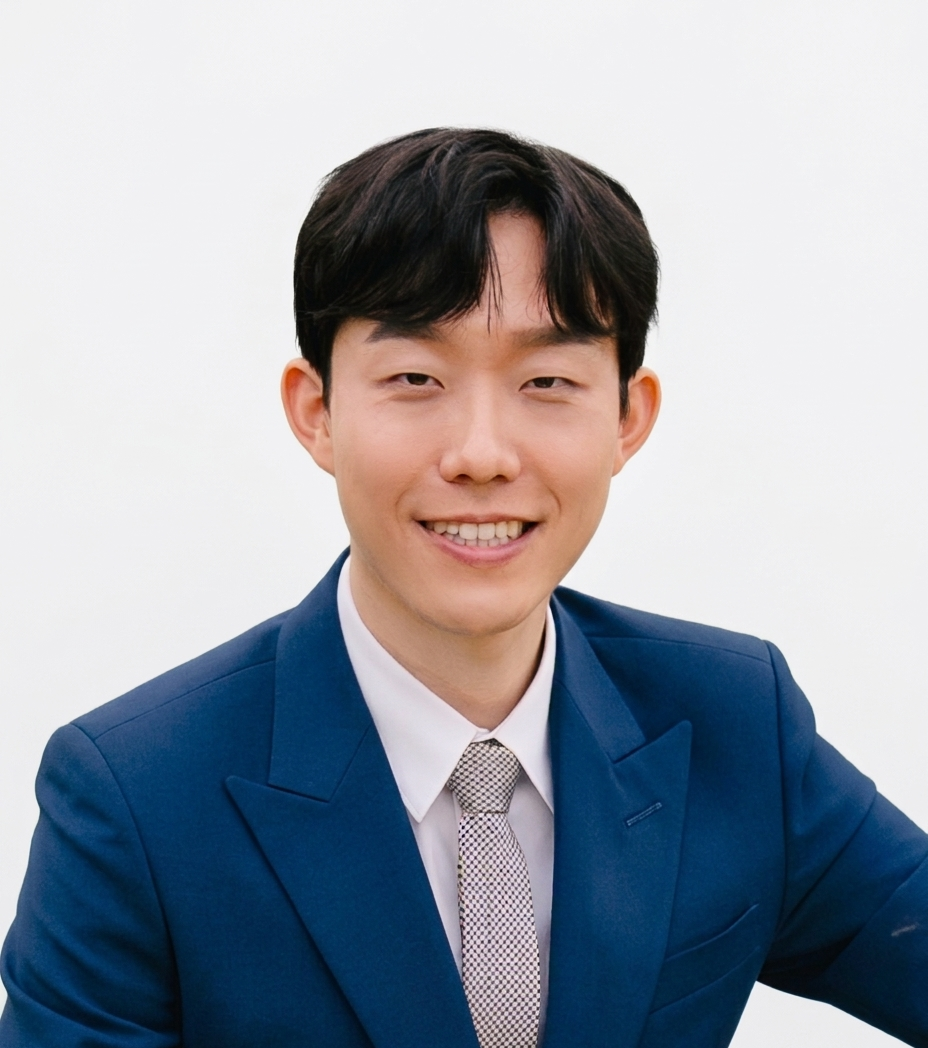
\includegraphics[width=2.4cm]{../profilepic/profile_pic_02_cropped.png}
\end{minipage}

%-----------Summary-----------------
\section{경력 요약}
\small{제약, 우주, AI 분야의 국제 R\&D 과제를 직접 이끌어 온 기술 중심의 프로젝트 매니저입니다. 현재 수백만 달러 규모 KEIT 동결건조 Digital Twin 과제의 미국 측을 총괄하고 있으며, 이전에는 3억 원 규모 정부 연구과제로 큐브위성 탑재체를 8년간 책임졌습니다. 프로젝트를 관리하는 것에 그치지 않고 필요한 소프트웨어를 직접 설계하고 구현합니다. 풀스택 웹 앱부터 실시간 Data Pipeline, ODE Simulation, 멀티에이전트 AI까지 직접 개발해 왔습니다. 한영 이중언어 구사가 가능하며 한미 양국 연구기관 간 기술 실무 조율 경험이 풍부합니다.}

%-----------Skills-----------------
\section{기술 역량}
  \resumeSubHeadingListStart
    \resumeSkills{\textbf{프로젝트 관리} -- WBS, Gantt Chart, Critical Path 분석, Risk 관리, Milestone 관리, 부서 간 조율, 정부과제 보고}
    \resumeSkills{\textbf{소프트웨어} -- Python, C/C++, MATLAB, FastAPI, Next.js, Docker, Git, Linux}
    \resumeSkills{\textbf{관리 도구} -- Excel WBS/Gantt, PowerPoint 현황 보고, Git/GitHub}
    \resumeSkills{\textbf{데이터/AI} -- PCA, PLS, ODE Modeling, TimescaleDB, Telegraf, 실시간 Data Pipeline}
    \resumeSkills{\textbf{하드웨어} -- 회로 설계, PCB Layout(KiCad), 센서 시스템, 임베디드 펌웨어, CAD(Fusion360, SolidWorks)}
  \resumeSubHeadingListEnd

%-----------PROJECT MANAGEMENT-----------------
\section{프로젝트 관리 경험}
  \resumeSubHeadingListStart

    \resumeSubheadingThree
      {매사추세츠 대학교 로웰 (KEIT 과제)}{미국 매사추세츠주 로웰}
      {PM 겸 기술 책임자 -- 동결건조 Digital Twin}{2025.07 -- 현재}
      {mRNA-LNP 제약 동결건조 공정 Digital Twin 개발, 6인 팀 총괄}{}
      \resumeItemListStart
        \resumeItem{KEIT 5개년 과제 미국 측 PM으로서 한국 파트너 기관과 공동 운영}
        \resumeItem{R\&D 3년 + 기술이전 2년, 총 2단계 15개 Work Package WBS 및 다년 Gantt 관리}
        \resumeItem{주간 현황 회의 주재, 경영진 보고, Milestone 점검, Risk 식별}
        \resumeItem{\$194K+ TDLAS 등 특수 장비 조달 Tracking 및 벤더 일정을 과제 일정에 연동}
        \resumeItem{실험, Modeling, Frontend, Backend 등 병렬 작업 흐름별 월간 목표 할당}
        \resumeItem{상용 도구(gPROMS) 한계로 Python 자체 개발로 전환, 일정 영향 없이 대응}
        \resumeItem{핵심 SW 직접 구현: 9-state ODE 모델, Multi-Agent AI(DAEMON), FastAPI + Next.js, Telegraf/TimescaleDB}
      \resumeItemListEnd

    \resumeSubheadingThree
      {고려대학교 (NRF + GPF 과제)}{서울}
      {PM 겸 기술 책임자 -- BioCubeSat 생물학 탑재체(CyanOx)}{2017.03 -- 2024.02}
      {정부과제 2건(GPF 5년 + NRF 3년), 총 3억 원(\textasciitilde\$230K) 규모}{}
      \resumeItemListStart
        \resumeItem{3U CubeSat 생물학 Payload를 8년에 걸쳐 기획부터 통합까지 총괄}
        \resumeItem{기구, 유체, 센서, 제어, MCU, 생물 6개 Subsystem WBS 작성, 12차 Action Plan 및 Gantt 운용}
        \resumeItem{4인 팀원별 월간 업무 배분, 매월 진척 보고서 수합 및 과제 현황 관리}
        \resumeItem{전체 연구비(인건비, 재료비, 장비비, 출장비) NRF/GPF 정산 기준에 맞춰 집행}
        \resumeItem{착수·연차(2건)·최종 보고서 각 5\textasciitilde 8차 수정 후 전량 통과}
        \resumeItem{주간 Team Meeting에서 Scope, Gantt, 개발 방법론, 월간 계획 점검}
        \resumeItem{6개 Subsystem 설계-제작-시험 Cycle을 2차 H/W 통합까지 조율}
        \resumeItem{과제 성과물로 제1저자 논문 3편 게재, 학회 발표 4건}
      \resumeItemListEnd

    \resumeSubheading
      {비영리 공동체}{서울}
      {공동 창립자 겸 총괄 운영자 -- 효과적 이타주의 한국 및 AMF Korea}{2015 -- 2023}
      \resumeItemListStart
        \resumeItem{2015년 EA Korea 공동 설립, 한영 이중 언어 공동체 구축 및 정기 모임·KPI 운영}
        \resumeItem{Centre for Effective Altruism으로부터 \$100K 이상 Grant 유치}
        \resumeItem{OKR, 회원 Pipeline, 재무, 프로젝트 Tracking, 표준 절차 등 조직 체계를 처음부터 설계}
        \resumeItem{북클럽, EA 자료 한국어 번역, Outreach, 회원 설문 등 다수 프로젝트 병행}
        \resumeItem{2023년 AMF Korea 사단법인 설립 지원, 이사진 모집 및 한영 법률 서류 작성}
      \resumeItemListEnd

  \resumeSubHeadingListEnd

%-----------EXPERIENCE-----------------
\section{경력 사항}
  \resumeSubHeadingListStart

    \resumeSubheading
      {매사추세츠 대학교 로웰}{미국 매사추세츠주 로웰}
      {Postdoctoral Associate -- 제조 공정 Monitoring 및 시험 자동화}{2025.07 -- 현재}
      \resumeItemListStart
        \resumeItem{상용 제품을 대체하는 Python 진단 SW를 개발하여 실시간 제조 공정 Monitoring 구현}
        \resumeItem{제약 생산 Batch 100건 이상 대상 이상 탐지 및 품질 예측 Pipeline 구축}
        \resumeItem{다일(多日) Batch 제조 주기에 데이터 기반 시험 전략 및 자동 Error Flagging 체계 도입}
        \resumeItem{유관 부서 요구사항을 표준화된 시험 절차서 및 문서로 정리}
      \resumeItemListEnd

    \resumeSubheading
      {한화시스템}{서울}
      {시스템 통합 Engineer -- 시험 장비 설계 및 위성 통합}{2024.02 -- 2025.05}
      \resumeItemListStart
        \resumeItem{위성 Subsystem FAT용 EGSE Architecture 설계 및 구축}
        \resumeItem{군용 SAR 위성 EM/QM/FM 단계별 System Level Test 계획 및 수행}
        \resumeItem{DAQ H/W, 센서 Interface, 전장 연결을 갖춘 Turnkey 시험 환경 납품}
        \resumeItem{통합 중 전기/기계 고장 Root Cause Analysis(RCA) 수행 및 시정조치 완료}
        \resumeItem{반복 고장 패턴 분석을 통한 Design for Testability(DFT) 개선안 도출}
        \resumeItem{기능시험 시스템 구매·통합·Commissioning 관리}
        \resumeItem{시험 절차서, Fixture 도면, Troubleshooting Guide 작성 및 유지}
        \resumeItem{Engineer 및 기술자 대상 시험 장비 운용·Debug 교육}
        \resumeItem{전기, 기계, SW, 사업관리 팀과 협업하여 시험 Coverage와 일정 조율}
      \resumeItemListEnd

  \resumeSubHeadingListEnd

%-----------EDUCATION-----------------
\section{학력}
  \resumeSubHeadingListStart
    \resumeSubheading
      {고려대학교}{서울}
      {전기공학 박사 -- 임베디드 센서 시스템 및 H/W Test 개발}{2017.03 -- 2024.02}
      \resumeItemListStart
        \resumeItem{CubeSat 생물학 Payload 개발을 위한 연구비 3억 원(\textasciitilde\$230K) 확보 및 집행}
        \resumeItem{Oscilloscope, DMM, Function Generator, Power Supply 등을 활용한 맞춤형 Test Fixture 및 DAQ 환경 구축}
        \resumeItem{Multi-Modal 센서 보드를 회로 설계부터 PCB 제작, 조립, 인증까지 Full Cycle 수행}
        \resumeItem{UART, SPI, I2C 기반 실시간 다채널 DAQ MCU Firmware를 C/C++로 개발}
        \resumeItem{환경시험·신뢰성시험 반복을 통해 Failure Mode를 파악하고 제작 조건 최적화}
        \resumeItem{H/W-F/W Interface 결함 진단 후 다수 Revision을 거쳐 해결}
        \resumeItem{센서, 시험 시스템, 우주 Payload 관련 제1저자 논문 3편, 공저 10편 이상 게재}
      \resumeItemListEnd
    \resumeSubheading
      {건국대학교}{서울}
      {기계공학 학사}{2013.03 -- 2017.02}
      \resumeItemListStart
        \resumeItem{전기화학 센서 미세가공, Cleanroom 공정, H/W Prototyping 연구}
        \resumeItem{CAD Modeling, 기계 조립, PCB 시작품 제작, 정밀 계측 실무 경험}
      \resumeItemListEnd
  \resumeSubHeadingListEnd

%-----------PUBLICATIONS-----------------
\section{논문 실적}
\subsection*{\normalsize 학술지 논문}
  \resumeSubHeadingListStart
    \resumeItem{\textbf{\underline{Saeyoung Kim}}, Jaewon Lee, Kimia Babaei, Seonkgyu Yoon, ``Digital Twins in Lyophilization: Advances in Pharmaceutical Process Development and Optimization,'' \textit{Biotechnology Advances}, 2026. (원고 준비 중, 투고 목표: 2026년 1분기)}
    \resumeItem{Jinhwee Kil, \textbf{\underline{Saeyoung Kim}}, James Jungho Pak, ``Investigation of thermal management strategies for biological CubeSat payloads,'' \textit{Acta Astronautica}, 2024, Art. no. 228.}
    \resumeItem{\textbf{\underline{Kim, S.}}; Park, S.; Pak, J.J., ``Multi-Modal Multi-Array Electrochemical and Optical Sensor Suite for a Biological CubeSat Payload,'' \textit{MDPI Sensors}, 2024, 24, Art. no. 265.}
    \resumeItem{Ji-Hoon Han, Sang Hyun Park, \textbf{\underline{Saeyoung Kim}}, James Jungho Pak, ``A Performance Improvement of Enzyme-Based Electrochemical Lactate Sensor Fabricated by Electroplating Novel PdCu Mediator on a Laser Induced Graphene Electrode,'' \textit{Bioelectrochemistry}, 2022, 148, 108259.}
    \resumeItem{\textbf{\underline{Saeyoung Kim}}, Ji-Hoon Han, Beelee Chua, James Jungho Pak, ``A pH Sensing Pipette for Cross-Contamination Prevention in Industrial Fermentation,'' \textit{IEEE Trans. Industrial Electronics}, 2022, 69(7), 7461-7469.}
    \resumeItem{S.D. Raut, N.M. Shinde, B.G. Ghule, \textbf{\underline{S. Kim}}, J.J. Pak, Q. Xia, R.S. Mane, ``Room-Temperature Solution Processed Sharp-Edged Nanoshapes of,'' \textit{Chemical Engineering Journal}, 2022, 433(2), 133627.}
    \resumeItem{S.E. Jeong, \textbf{\underline{S. Kim}}, J.H. Han, J. Jungho Pak, ``Simple Laser-Induced Graphene Fiber Electrode Fabrication for High-Performance Heavy-Metal Sensing,'' \textit{Microchemical Journal}, 2022, 172, 106950.}
    \resumeItem{Sanghoon Cho, Jungmo Jung, \textbf{\underline{Saeyoung Kim}}, James Pak, ``Conduction Mechanism and Synaptic Behaviour of Interfacial Switching AlOσ-based RRAM,'' \textit{Semiconductor Science and Technology}, 2020, 35(8), 085006.}
    \resumeItem{Ji-Hoon Han, \textbf{\underline{Saeyoung Kim}}, Jaesung Choi, Sora Kang, Youngmi Kim Pak, James Jungho Pak, ``Development of Multi-Well-Based Electrochemical Dissolved Oxygen Sensor Array,'' \textit{Sensors and Actuators B: Chemical}, 2020, 306, 127465.}
  \resumeSubHeadingListEnd

\subsection*{\normalsize 학회 발표}
  \resumeSubHeadingListStart
    \resumeItem{\textit{Thermal Management System for a Fluidic Card in a Small Satellite Biological Payload}, 대한전기학회 추계학술대회, 2022.}
    \resumeItem{\textit{A Pipette with an Integrated pH Sensor for Liquid Sampling Applications}, 대한전기학회 하계학술대회, 2019.}
    \resumeItem{\textit{IoT System for Monitoring pH, Dissolved Oxygen, Temperature, and Electrical Conductivity in Liquids}, 대한전기학회 하계학술대회, 2018.}
    \resumeItem{\textit{Development Trends of Non-Invasive Glucose Sensor Technology}, 대한전기학회 하계학술대회, 2017.}
  \resumeSubHeadingListEnd

\subsection*{\normalsize 세미나 발표}
  \resumeSubHeadingListStart
    \resumeItem{\textit{Bioprocessing in Space: Challenges and Opportunities for Pharmaceutical Manufacturing Beyond Earth}, LoCSST, UMass Lowell, 2025.}
  \resumeSubHeadingListEnd

%-------------------------------------------
\end{document}
